\documentclass[ignorenonframetext,]{beamer}
\setbeamertemplate{caption}[numbered]
\setbeamertemplate{caption label separator}{: }
\setbeamercolor{caption name}{fg=normal text.fg}
\beamertemplatenavigationsymbolsempty
\usepackage{lmodern}
\usepackage{amssymb,amsmath}
\usepackage{ifxetex,ifluatex}
\usepackage{fixltx2e} % provides \textsubscript
\ifnum 0\ifxetex 1\fi\ifluatex 1\fi=0 % if pdftex
  \usepackage[T1]{fontenc}
  \usepackage[utf8]{inputenc}
\else % if luatex or xelatex
  \ifxetex
    \usepackage{mathspec}
  \else
    \usepackage{fontspec}
  \fi
  \defaultfontfeatures{Ligatures=TeX,Scale=MatchLowercase}
\fi
\usefonttheme{structurebold}
% use upquote if available, for straight quotes in verbatim environments
\IfFileExists{upquote.sty}{\usepackage{upquote}}{}
% use microtype if available
\IfFileExists{microtype.sty}{%
\usepackage{microtype}
\UseMicrotypeSet[protrusion]{basicmath} % disable protrusion for tt fonts
}{}
\newif\ifbibliography
\usepackage{color}
\usepackage{fancyvrb}
\newcommand{\VerbBar}{|}
\newcommand{\VERB}{\Verb[commandchars=\\\{\}]}
\DefineVerbatimEnvironment{Highlighting}{Verbatim}{commandchars=\\\{\}}
% Add ',fontsize=\small' for more characters per line
\usepackage{framed}
\definecolor{shadecolor}{RGB}{248,248,248}
\newenvironment{Shaded}{\begin{snugshade}}{\end{snugshade}}
\newcommand{\KeywordTok}[1]{\textcolor[rgb]{0.13,0.29,0.53}{\textbf{{#1}}}}
\newcommand{\DataTypeTok}[1]{\textcolor[rgb]{0.13,0.29,0.53}{{#1}}}
\newcommand{\DecValTok}[1]{\textcolor[rgb]{0.00,0.00,0.81}{{#1}}}
\newcommand{\BaseNTok}[1]{\textcolor[rgb]{0.00,0.00,0.81}{{#1}}}
\newcommand{\FloatTok}[1]{\textcolor[rgb]{0.00,0.00,0.81}{{#1}}}
\newcommand{\ConstantTok}[1]{\textcolor[rgb]{0.00,0.00,0.00}{{#1}}}
\newcommand{\CharTok}[1]{\textcolor[rgb]{0.31,0.60,0.02}{{#1}}}
\newcommand{\SpecialCharTok}[1]{\textcolor[rgb]{0.00,0.00,0.00}{{#1}}}
\newcommand{\StringTok}[1]{\textcolor[rgb]{0.31,0.60,0.02}{{#1}}}
\newcommand{\VerbatimStringTok}[1]{\textcolor[rgb]{0.31,0.60,0.02}{{#1}}}
\newcommand{\SpecialStringTok}[1]{\textcolor[rgb]{0.31,0.60,0.02}{{#1}}}
\newcommand{\ImportTok}[1]{{#1}}
\newcommand{\CommentTok}[1]{\textcolor[rgb]{0.56,0.35,0.01}{\textit{{#1}}}}
\newcommand{\DocumentationTok}[1]{\textcolor[rgb]{0.56,0.35,0.01}{\textbf{\textit{{#1}}}}}
\newcommand{\AnnotationTok}[1]{\textcolor[rgb]{0.56,0.35,0.01}{\textbf{\textit{{#1}}}}}
\newcommand{\CommentVarTok}[1]{\textcolor[rgb]{0.56,0.35,0.01}{\textbf{\textit{{#1}}}}}
\newcommand{\OtherTok}[1]{\textcolor[rgb]{0.56,0.35,0.01}{{#1}}}
\newcommand{\FunctionTok}[1]{\textcolor[rgb]{0.00,0.00,0.00}{{#1}}}
\newcommand{\VariableTok}[1]{\textcolor[rgb]{0.00,0.00,0.00}{{#1}}}
\newcommand{\ControlFlowTok}[1]{\textcolor[rgb]{0.13,0.29,0.53}{\textbf{{#1}}}}
\newcommand{\OperatorTok}[1]{\textcolor[rgb]{0.81,0.36,0.00}{\textbf{{#1}}}}
\newcommand{\BuiltInTok}[1]{{#1}}
\newcommand{\ExtensionTok}[1]{{#1}}
\newcommand{\PreprocessorTok}[1]{\textcolor[rgb]{0.56,0.35,0.01}{\textit{{#1}}}}
\newcommand{\AttributeTok}[1]{\textcolor[rgb]{0.77,0.63,0.00}{{#1}}}
\newcommand{\RegionMarkerTok}[1]{{#1}}
\newcommand{\InformationTok}[1]{\textcolor[rgb]{0.56,0.35,0.01}{\textbf{\textit{{#1}}}}}
\newcommand{\WarningTok}[1]{\textcolor[rgb]{0.56,0.35,0.01}{\textbf{\textit{{#1}}}}}
\newcommand{\AlertTok}[1]{\textcolor[rgb]{0.94,0.16,0.16}{{#1}}}
\newcommand{\ErrorTok}[1]{\textcolor[rgb]{0.64,0.00,0.00}{\textbf{{#1}}}}
\newcommand{\NormalTok}[1]{{#1}}
\usepackage{graphicx,grffile}
\makeatletter
\def\maxwidth{\ifdim\Gin@nat@width>\linewidth\linewidth\else\Gin@nat@width\fi}
\def\maxheight{\ifdim\Gin@nat@height>\textheight0.8\textheight\else\Gin@nat@height\fi}
\makeatother
% Scale images if necessary, so that they will not overflow the page
% margins by default, and it is still possible to overwrite the defaults
% using explicit options in \includegraphics[width, height, ...]{}
\setkeys{Gin}{width=\maxwidth,height=\maxheight,keepaspectratio}

% Prevent slide breaks in the middle of a paragraph:
\widowpenalties 1 10000
\raggedbottom

\AtBeginPart{
  \let\insertpartnumber\relax
  \let\partname\relax
  \frame{\partpage}
}
\AtBeginSection{
  \ifbibliography
  \else
    \let\insertsectionnumber\relax
    \let\sectionname\relax
    \frame{\sectionpage}
  \fi
}
\AtBeginSubsection{
  \let\insertsubsectionnumber\relax
  \let\subsectionname\relax
  \frame{\subsectionpage}
}

\setlength{\emergencystretch}{3em}  % prevent overfull lines
\providecommand{\tightlist}{%
  \setlength{\itemsep}{0pt}\setlength{\parskip}{0pt}}
\setcounter{secnumdepth}{0}
\definecolor{links}{HTML}{800080}
\hypersetup{colorlinks,linkcolor=,urlcolor=links}

\title{Web Data Collection with R}
\subtitle{OAuth API Case Study}
\author{Peter Meißner / 2016-02-29 -- 2016-03-04 / ECPR WSMT}
\date{}

\begin{document}
\frame{\titlepage}

\begin{frame}
\tableofcontents[hideallsubsections]
\end{frame}

\section{Twitter API - API with
authentication}\label{twitter-api---api-with-authentication}

\begin{frame}{API with authentication}

\begin{itemize}
\tightlist
\item
  provides API for tweeting, accessing tweets and user information
\item
  more complex interface
\item
  access needs Oauth authentication

  \begin{itemize}
  \tightlist
  \item
    get account / developer account
  \item
    create/register application
  \item
    use credentials to authorize
  \end{itemize}
\end{itemize}

\end{frame}

\begin{frame}{API with authentication}

\begin{itemize}
\tightlist
\item
  \emph{{[}httr{]}} has capabilities and some examples:
  \url{https://github.com/hadley/httr/tree/master/demo}
\item
  use an already written package
\item
  \ldots{} twitteR package by Jeff Gentry (!must read!:
  \url{http://geoffjentry.hexdump.org/twitteR.pdf})
\end{itemize}

\end{frame}

\begin{frame}{OAuth}

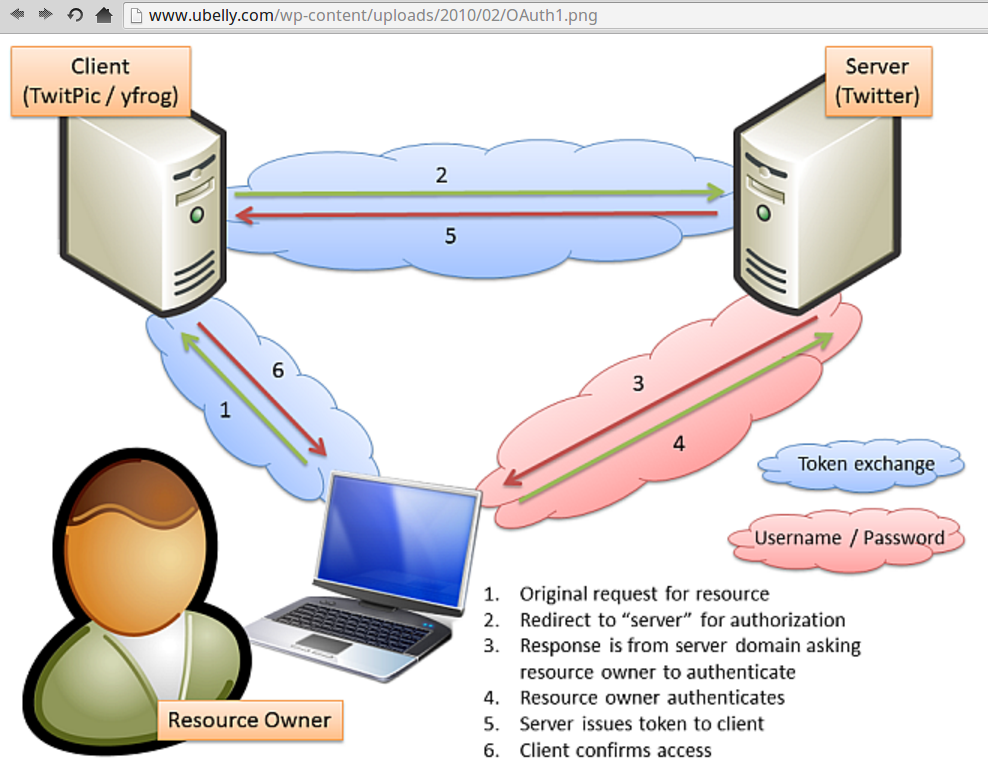
\includegraphics{fig/oauth.png}

\end{frame}

\begin{frame}{twitter app}

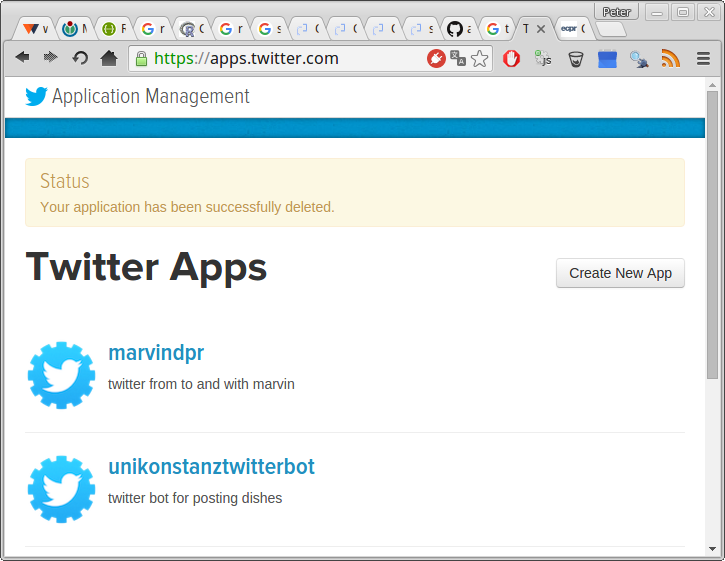
\includegraphics{fig/twitterapp1.png}

\end{frame}

\begin{frame}{twitter app}

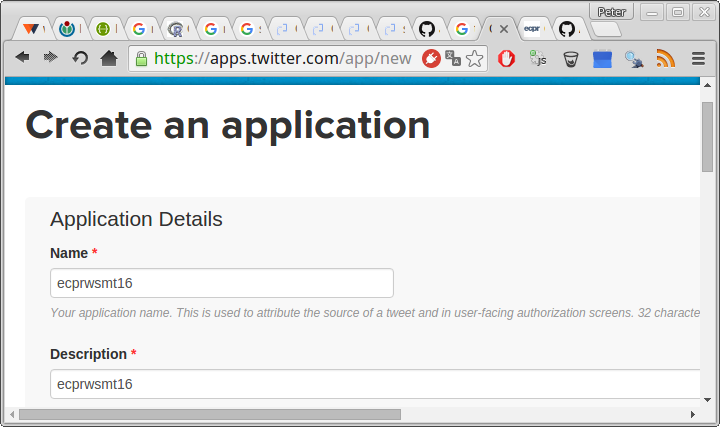
\includegraphics{fig/twitterapp2.png}

\end{frame}

\begin{frame}{twitter app}

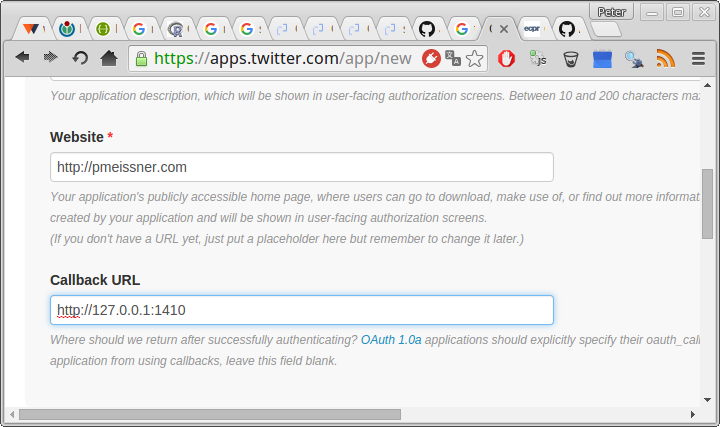
\includegraphics{fig/twitterapp3.png}

\end{frame}

\begin{frame}{twitter app}


\includegraphics{fig/twitterapp4.png}

\end{frame}

\begin{frame}{twitter app}

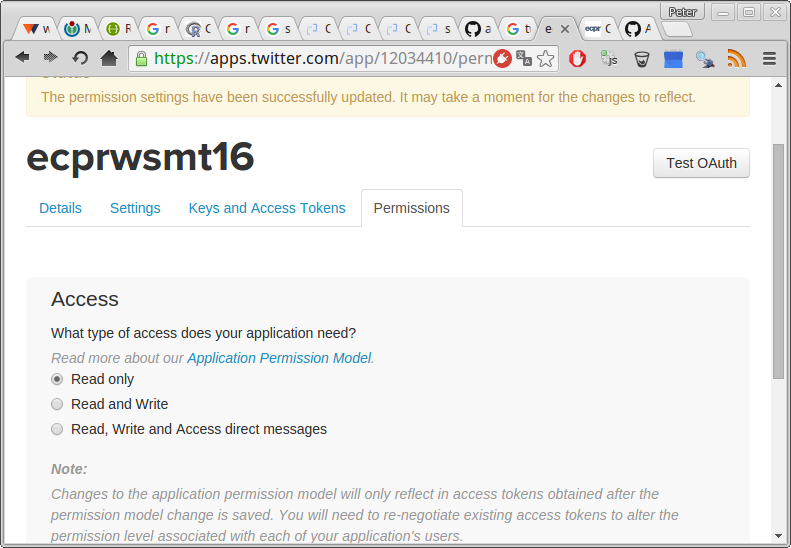
\includegraphics{fig/twitterapp5.png}

\end{frame}

\begin{frame}{twitter app}

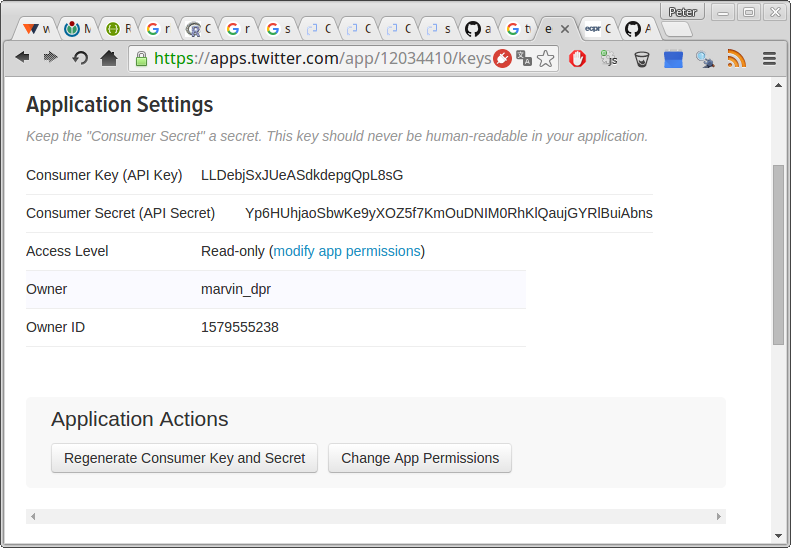
\includegraphics{fig/twitterapp6.png}

\end{frame}

\begin{frame}{twitter app}

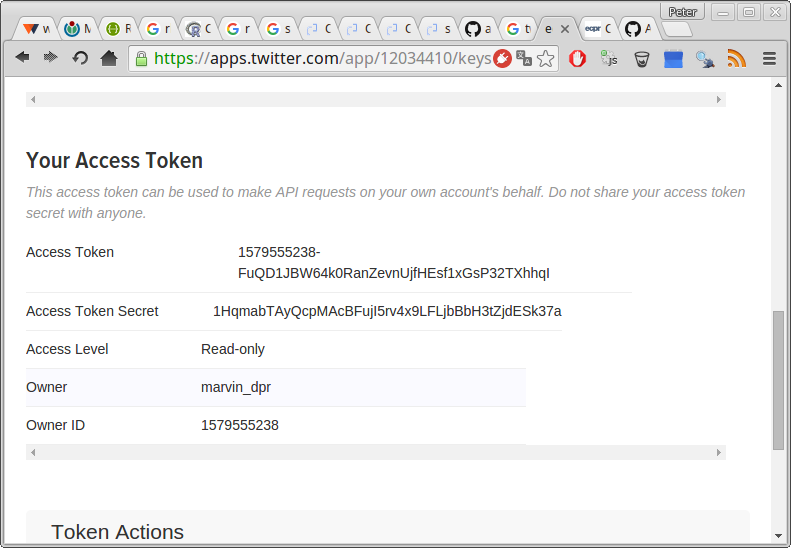
\includegraphics{fig/twitterapp7.png}

\end{frame}

\begin{frame}[fragile]{the twitter example}

\begin{Shaded}
\begin{Highlighting}[]
\CommentTok{# packages}
\KeywordTok{library}\NormalTok{(httr)}
\KeywordTok{library}\NormalTok{(dplyr)}
\KeywordTok{library}\NormalTok{(magrittr)}
\KeywordTok{library}\NormalTok{(stringr)}
\CommentTok{# credentials}
\NormalTok{cred_file <-}\StringTok{ "ecpr_wsmt_2016.credentials"}
\NormalTok{tmp       <-}\StringTok{ }\KeywordTok{readLines}\NormalTok{(cred_file)}
\NormalTok{tmp}
\end{Highlighting}
\end{Shaded}

\begin{verbatim}
## [1] "twitter_api_key=LLDebjSxJUeASdkdepgQpL8sG"                                
## [2] "twitter_api_secret=Yp6HUhjaoSbwKe9yXOZ5f7KmOuDNIM0RhKlQaujGYRlBuiAbns"    
## [3] "twitter_access_token=1579555238-FuQD1JBW64k0RanZevnUjfHEsf1xGsP32TXhhqI"  
## [4] "twitter_access_token_secret=1HqmabTAyQcpMAcBFujI5rv4x9LFLjbBbH3tZjdESk37a"
\end{verbatim}

\end{frame}

\begin{frame}[fragile]{the twitter example}

\begin{Shaded}
\begin{Highlighting}[]
\NormalTok{key =}\StringTok{ }\NormalTok{stringr::}\KeywordTok{str_replace}\NormalTok{(}
  \KeywordTok{grep}\NormalTok{(}\StringTok{"twitter_api_key="}\NormalTok{, tmp, }\DataTypeTok{value =} \NormalTok{T), }
  \StringTok{"twitter_api_key="}\NormalTok{, }\StringTok{""}\NormalTok{)}

\NormalTok{secret =}\StringTok{ }\NormalTok{stringr::}\KeywordTok{str_replace}\NormalTok{(}
  \KeywordTok{grep}\NormalTok{(}\StringTok{"twitter_api_secret="}\NormalTok{, tmp, }\DataTypeTok{value =} \NormalTok{T), }
  \StringTok{"twitter_api_secret="}\NormalTok{, }\StringTok{""}\NormalTok{)}

\NormalTok{token =}\StringTok{ }\NormalTok{stringr::}\KeywordTok{str_replace}\NormalTok{(}
  \KeywordTok{grep}\NormalTok{(}\StringTok{"twitter_access_token="}\NormalTok{, tmp, }\DataTypeTok{value =} \NormalTok{T), }
  \StringTok{"twitter_access_token="}\NormalTok{, }\StringTok{""}\NormalTok{)}

\NormalTok{token_secret =}\StringTok{ }\NormalTok{stringr::}\KeywordTok{str_replace}\NormalTok{(}
  \KeywordTok{grep}\NormalTok{(}\StringTok{"twitter_access_token_secret="}\NormalTok{, tmp, }\DataTypeTok{value =} \NormalTok{T), }
  \StringTok{"twitter_access_token_secret="}\NormalTok{, }\StringTok{""}\NormalTok{)}
\end{Highlighting}
\end{Shaded}

\end{frame}

\begin{frame}[fragile]{the twitter example}

\begin{Shaded}
\begin{Highlighting}[]
\NormalTok{twitter_token <-}
\StringTok{  }\NormalTok{Token1}\FloatTok{.0}\NormalTok{$}\KeywordTok{new}\NormalTok{(}
    \DataTypeTok{endpoint      =} \OtherTok{NULL}\NormalTok{,}
    \DataTypeTok{params        =} \KeywordTok{list}\NormalTok{(}\DataTypeTok{as_header =} \OtherTok{TRUE}\NormalTok{),}
    \DataTypeTok{app           =} \KeywordTok{oauth_app}\NormalTok{( }\StringTok{"twitter"}\NormalTok{, key, secret ),}
    \DataTypeTok{credentials   =} \KeywordTok{list}\NormalTok{(}
      \DataTypeTok{oauth_token        =} \NormalTok{token,}
      \DataTypeTok{oauth_token_secret =} \NormalTok{token_secret}
    \NormalTok{)}
  \NormalTok{)}
\end{Highlighting}
\end{Shaded}

\end{frame}

\begin{frame}[fragile]{the twitter example}

\begin{Shaded}
\begin{Highlighting}[]
\NormalTok{req <-}
\StringTok{  }\KeywordTok{GET}\NormalTok{(}
    \KeywordTok{paste0}\NormalTok{(}
      \StringTok{"https://api.twitter.com/1.1/search/tweets.json"}\NormalTok{,}
      \StringTok{"?q=%23wsmt16&result_type=recent&count=100"}
    \NormalTok{),}
    \KeywordTok{config}\NormalTok{(}\DataTypeTok{token =} \NormalTok{twitter_token)}
  \NormalTok{)}
\end{Highlighting}
\end{Shaded}

\end{frame}

\begin{frame}[fragile]{the twitter example}

\begin{Shaded}
\begin{Highlighting}[]
\NormalTok{tweets <-}
\StringTok{  }\NormalTok{req %>%}
\StringTok{  }\KeywordTok{content}\NormalTok{(}\StringTok{"parsed"}\NormalTok{) %>%}
\StringTok{  }\KeywordTok{extract2}\NormalTok{(}\StringTok{"statuses"}\NormalTok{) %>%}
\StringTok{  }\KeywordTok{lapply}\NormalTok{(}\StringTok{`}\DataTypeTok{[}\StringTok{`}\NormalTok{, }\StringTok{"text"}\NormalTok{) %>%}
\StringTok{  }\KeywordTok{unlist}\NormalTok{(}\DataTypeTok{use.names=}\OtherTok{FALSE}\NormalTok{)}
\end{Highlighting}
\end{Shaded}

\end{frame}

\begin{frame}[fragile]{the twitter example}

\begin{Shaded}
\begin{Highlighting}[]
\NormalTok{tweets %>%}\StringTok{ }\KeywordTok{grep}\NormalTok{(}\StringTok{"^RT "}\NormalTok{,. ,}\DataTypeTok{invert=}\OtherTok{TRUE}\NormalTok{, }\DataTypeTok{value=}\OtherTok{TRUE}\NormalTok{) }
\end{Highlighting}
\end{Shaded}

\begin{verbatim}
##  [1] "@EJPRjournal special issue on qualitative research free\nto access now https://t.co/fhjCSzCLrh - could be interesting for those at #wsmt16"    
##  [2] "Is it that strong? What part of politics is not about relations between actors/groups/states? #wsmt16 https://t.co/PgXgGoiZrb"                 
##  [3] "Professional development course for instructors on empirical beer research at the @ECPR #wsmt16 https://t.co/xn4DckhmPC"                       
##  [4] "Advanced network analysis after hours at the @ECPR Winter School in Methods and Techniques #wsmt16 https://t.co/GRpjv2nMzf"                    
##  [5] "Sitting in a beer tasting with 20 methods and statistics teachers feels like an episode of @partiallyd #wsmt16"                                
##  [6] "Back in the student seat #wsmt16"                                                                                                              
##  [7] "Best about teaching? Coming up with examples ... #wsmt16 #rstats @ecpr https://t.co/yooxkoc3rW"                                                
##  [8] "\"#polsci is inherently relational\" - strong thesis by P. Leifeld in the brownbagsession on #SNA @ECPR Winter School #wsmt16"                 
##  [9] "SNA frontiers and case-oriented research complexities on the menu for today’s Brown Bags #WSMT16 – enjoy! https://t.co/ZiB3UQB5e4"             
## [10] "Lasse Gerrits, Marie Østergaard Møller and Derek Beach will discuss Complexity in Case-oriented Research #wsmt16 #BrownBagLunchSession"        
## [11] "Prof. Lasse Gerrits will join the Brown Bag Lunch Session at @ECPR winter school on methods + techniques today. Room F135 at 12:45 #wsmt16"    
## [12] "My verdict on smoke beer: it's like multilevel models: it works, but not for every occasion #wsmt16 #1stdaylesson https://t.co/bBJmQCUnId"     
## [13] "No social event without self references! #wsmt16 @ecpr @ComparPol @miriboehme @littvay @felixhaass @DominikVogel86 https://t.co/45u9Z04XZ0"    
## [14] "Let it snow, let it snow, let it snow @ECPR #wsmt16 https://t.co/bFCR3nSS39"                                                                   
## [15] "I know it's winter school but does it really have to snow... #wsmt16 #bamberg #methods #polisci https://t.co/mZNwGYu2yD"                       
## [16] "If you're at the #wsmt16 don't miss the Brown Bag Lunch Sessions tomorrow at 12:45. For details, see the website https://t.co/mxHvCBbjik"      
## [17] "The 2016 ECPR Winter School is now in full swing! Don't forget to send us your pictures and updates using #wsmt16"                             
## [18] "Lots of levels, lots of interesting projects in @littvay &amp; @cmbosancianu 's multilevel class. Looking forward to rest of the week. #wsmt16"
## [19] "Welcome to over 400 participants and instructors attending the @ECPR Winter School in Methods and Techniques in Bamberg @Bamberg_de #wsmt16"   
## [20] "Looking forward to participate in #wsmt16  course on SEM. Starts tomorrow."                                                                    
## [21] "#wsmt16 here I come. Two hours late because of a theft at the train station and without all my books and preparation proof. But I'll b there"  
## [22] "Just arrived for @ECPR Winter school in Bamberg! Good to be back in Germany! #wsmt16"                                                          
## [23] "Troubleshooting LaTeX at the @ECPR #WSMT16 food and drinks reception with @cmbosancianu and @CarstenQSchneid https://t.co/NiqdiAVdke"          
## [24] "Temporary office for the week. Hallohhh Bamberg @ECPR #wsmt16 https://t.co/VJtiM5E0SP"                                                         
## [25] "I am excited to be back at @BAGSS5 for @ECPR #wsmt16, teaching course on #multimethod research. I'll pass on Rauchbier this year"              
## [26] "On my way. Going slowly but steady with Diesel-powered. @marvin_dpr @ecpr #wsmt16"                                                             
## [27] "On my way to Bamberg for the #wsmt16 @ECPR"                                                                                                    
## [28] "Preparing the Advanced Process-Tracing Methods Course for #wsmt16 @ECPR which starts on Monday! Looking forward to it!"                        
## [29] "Looking forward to today's course on #NVivo software at #wsmt16"                                                                               
## [30] "The 2016 ECPR Winter School starts tomorrow! If you're attending, please send us updates and pictures using the hashtag #wsmt16"               
## [31] "The 2016 ECPR Winter School starts this Friday! Let us know if you're attending by using the hashtag #wsmt16"
\end{verbatim}

\end{frame}

\end{document}
